\documentclass[11pt]{article}
\usepackage[utf8]{inputenc}	% Para caracteres en español
\usepackage{amsmath,amsthm,amsfonts,amssymb,amscd}
\usepackage{multirow,booktabs}
\usepackage[table]{xcolor}
\usepackage{fullpage}
\usepackage{lastpage}
\usepackage{enumitem}
\usepackage{fancyhdr}
\usepackage{mathrsfs}
\usepackage{wrapfig}
\usepackage{setspace}
\usepackage{calc}
\usepackage{multicol}
\usepackage{cancel}
\usepackage[retainorgcmds]{IEEEtrantools}
\usepackage[margin=1cm]{geometry}
\usepackage{amsmath}
\newlength{\tabcont}
\setlength{\parindent}{0.0in}
\setlength{\parskip}{0.05in}
\usepackage{empheq}
\usepackage{framed}
\usepackage[most]{tcolorbox}
\usepackage{xcolor}
\usepackage{graphicx}
\usepackage{listings}
% -- Basic formatting
\usepackage[utf8]{inputenc}
\usepackage[english]{babel}
\usepackage{times}
\usepackage{caption}
\usepackage{subcaption}
\usepackage{placeins}
\setlength{\parindent}{0pt}
\usepackage{indentfirst}% -- Defining colors:
\usepackage[dvipsnames]{xcolor}
\definecolor{codegreen}{rgb}{0,0.6,0}
\definecolor{codegray}{rgb}{0.5,0.5,0.5}
\definecolor{codepurple}{rgb}{0.58,0,0.82}
\definecolor{backcolour}{rgb}{0.95,0.95,0.92}% Definig a custom style:
\lstdefinestyle{mystyle}{
    backgroundcolor=\color{backcolour},   
    commentstyle=\color{codepurple},
    keywordstyle=\color{NavyBlue},
    numberstyle=\tiny\color{codegray},
    stringstyle=\color{codepurple},
    basicstyle=\ttfamily\footnotesize\bfseries,
    breakatwhitespace=false,         
    breaklines=true,                 
    captionpos=t,                    
    keepspaces=true,                 
    numbers=left,                    
    numbersep=5pt,                  
    showspaces=false,                
    showstringspaces=false,
    showtabs=false,                  
    tabsize=2
}% -- Setting up the custom style:
\lstset{style=mystyle}
\lstset{
  style=mystyle,
  framexleftmargin=3.5mm,
  rulesepcolor=\color{black},
  linewidth=0.6\linewidth,
  xleftmargin=12pt,
  aboveskip=12pt,
  belowskip=12pt
}
\colorlet{shadecolor}{orange!15}
\parindent 0in
\parskip 1pt
\geometry{margin=1in, headsep=0.25in}
\theoremstyle{definition}
\newtheorem{defn}{Definition}
\newtheorem{reg}{Rule}
\newtheorem{exer}{Exercise}
\newtheorem{note}{Note}
\graphicspath{ {./images/} }
\begin{document}
\setcounter{section}{0}
\title{MIE223 Lecture Notes}

\thispagestyle{empty}

\begin{center}
{\LARGE \bf Feature Analysis and Visualization}\\
{\large MIE223}\\
Winter 2025
\end{center}
\section{Feature Analysis and Visualization}
\subsection{Exploratory Data Analysis (EDA)}
John Tukey (Bell Labs, 1970’s) (Inventor of the box-plot)
\begin{itemize}
  \item The first time corporations had a lot of digital data
  \item Data on semiconductor processes, networks
\end{itemize}

Observed that statistics was preoccupied with
hypothesis testing
\begin{itemize}
  \item But there were no established methodologies for
  \textbf{generating (data-driven) hypotheses}
  \item Espoused a visual methodology and a new language
  S (R became the free version)
\end{itemize}
\subsection{Data Science Process}
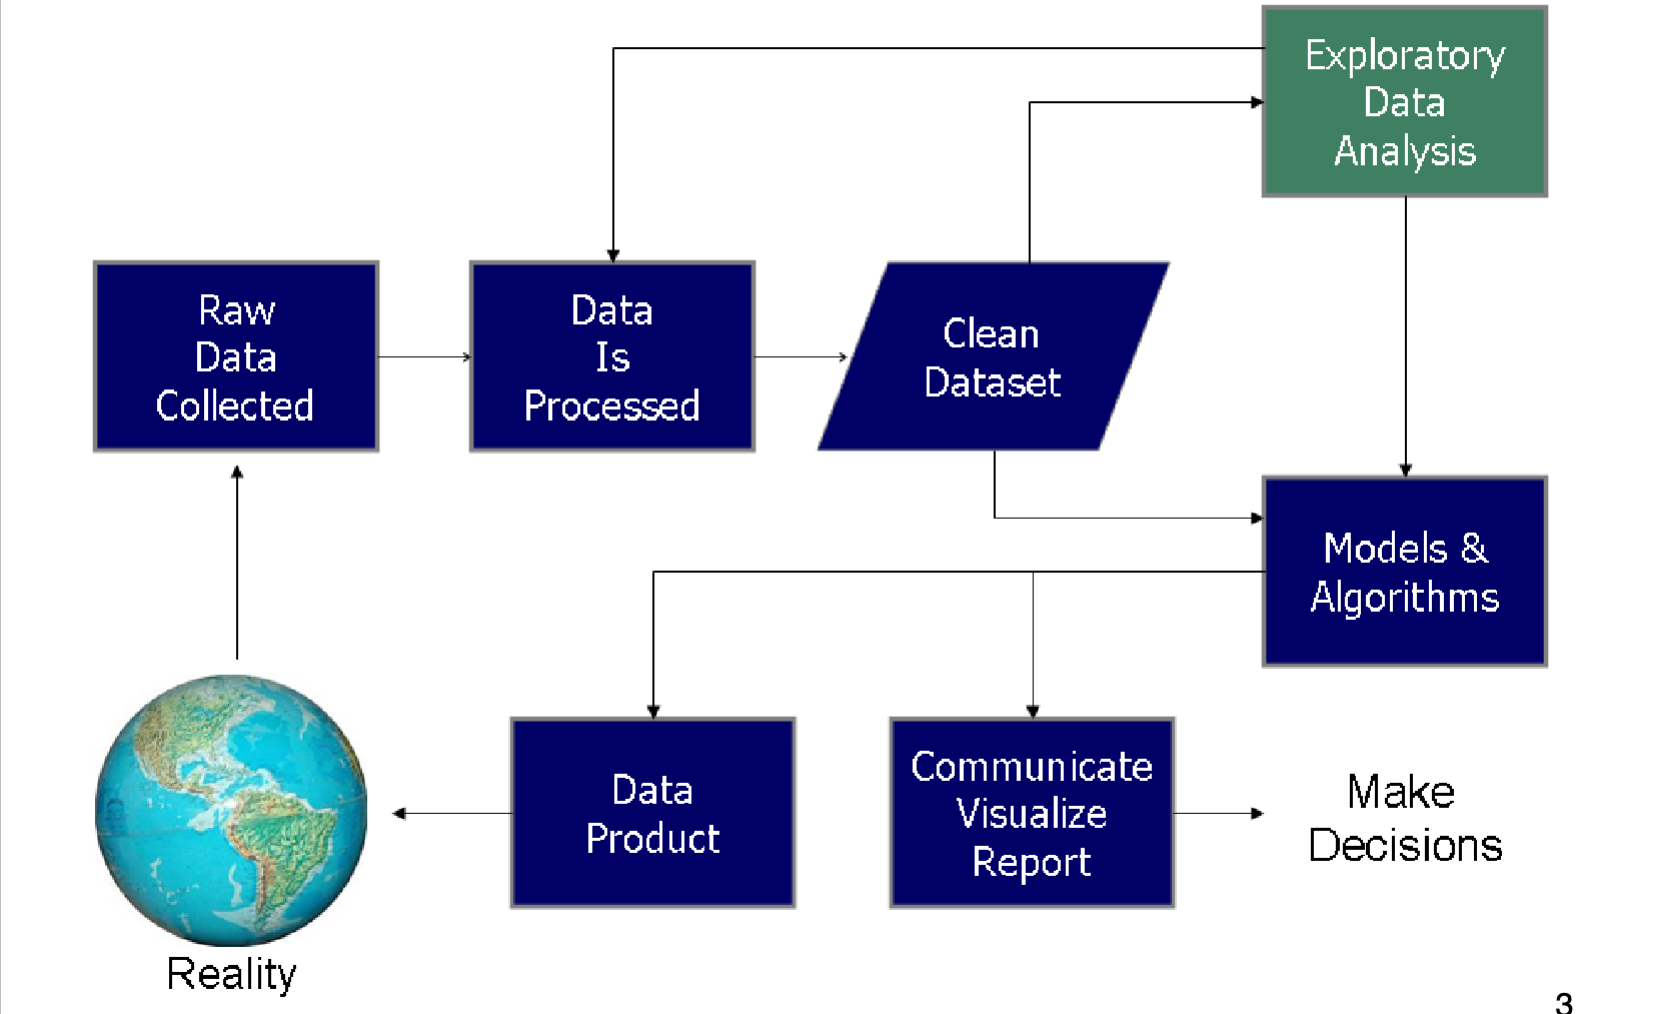
\includegraphics[width=\textwidth]{1.png}

\subsection{Data Cleaning: Brief Recap}
~80\% of your Data Science time

Some pointers:
\begin{itemize}
  \item Missing values – do not
  replace with 0 or -999
  \item Treat as missing
  \item Look for frequencies of
  values or outliers (-999)
  \begin{itemize}
    \item \textbf{Histograms} invaluable
    \item Examine \textbf{outliers} 
  \end{itemize}
  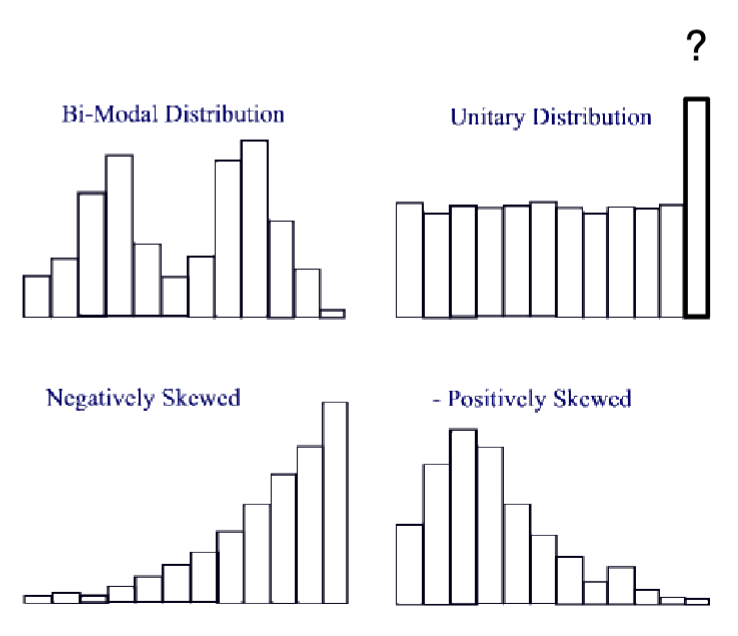
\includegraphics[width=\textwidth-27.37506pt]{2.png}
\end{itemize}
\section{Correlation}
We’ll be look at feature distributions
independently (per column), but also
relationships between features (columns).
Correlation is one of the first tools you think of
for looking at the relationship between two
features (but has limitations)
\subsection{Correlated variables}
Two variables are correlated if changes in one
variable, correspond to changes in the other

Correlation in general refers to the statistical
association between two variables
\begin{itemize}
  \item This statistical association allows us to make
  estimates for the one variable based on the value of
  the other
  \item While we typically think of linear relationships
  between variables, nonlinear might exist too
\end{itemize}
\subsection{Linear correlation}
\begin{itemize}
  \item Two variables x and y are said to be
  linearly correlated if their relationship can
  be described by the following equation:
\end{itemize}
\begin{equation}
  y = \alpha + \beta x, \beta \neq 0
\end{equation}
\begin{itemize}
  \item This relationship will not be exact
  \item There will be an error associated with it, and
  hence, in reality:
  \item $\epsilon$ is the error term for the relationship
\end{itemize}
\begin{equation}
  y = \alpha + \beta x + \epsilon, \beta \neq 0
\end{equation}
\subsection{Pearson correlation coefficient}
\begin{itemize}
  \item In order to test the linear association
  between two variables x and y we can use
  the Pearson correlation coefficient r$_{xy}$

  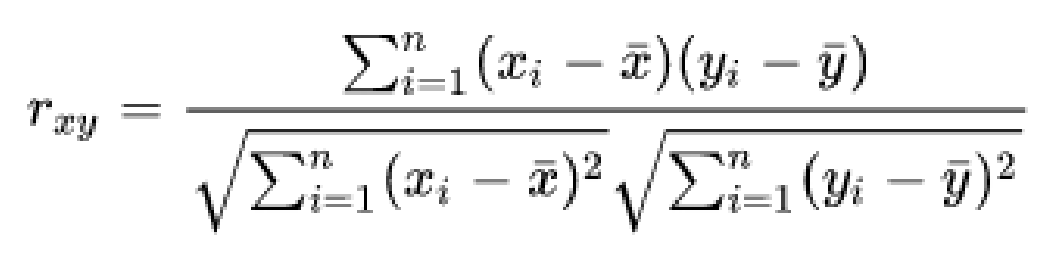
\includegraphics[width=\textwidth/2]{3.png}
  \item Pearson correlation is in the range [-1,1]
  \begin{itemize}
    \item 1: perfect/strong and positive linear correlation
    \item -1: perfect/strong and negative linear correlation
    \item 0: no linear correlation
  \end{itemize}
  \item It is very crucial to understand that this
  correlation coefficient can only examine
  linear associations between two variables

  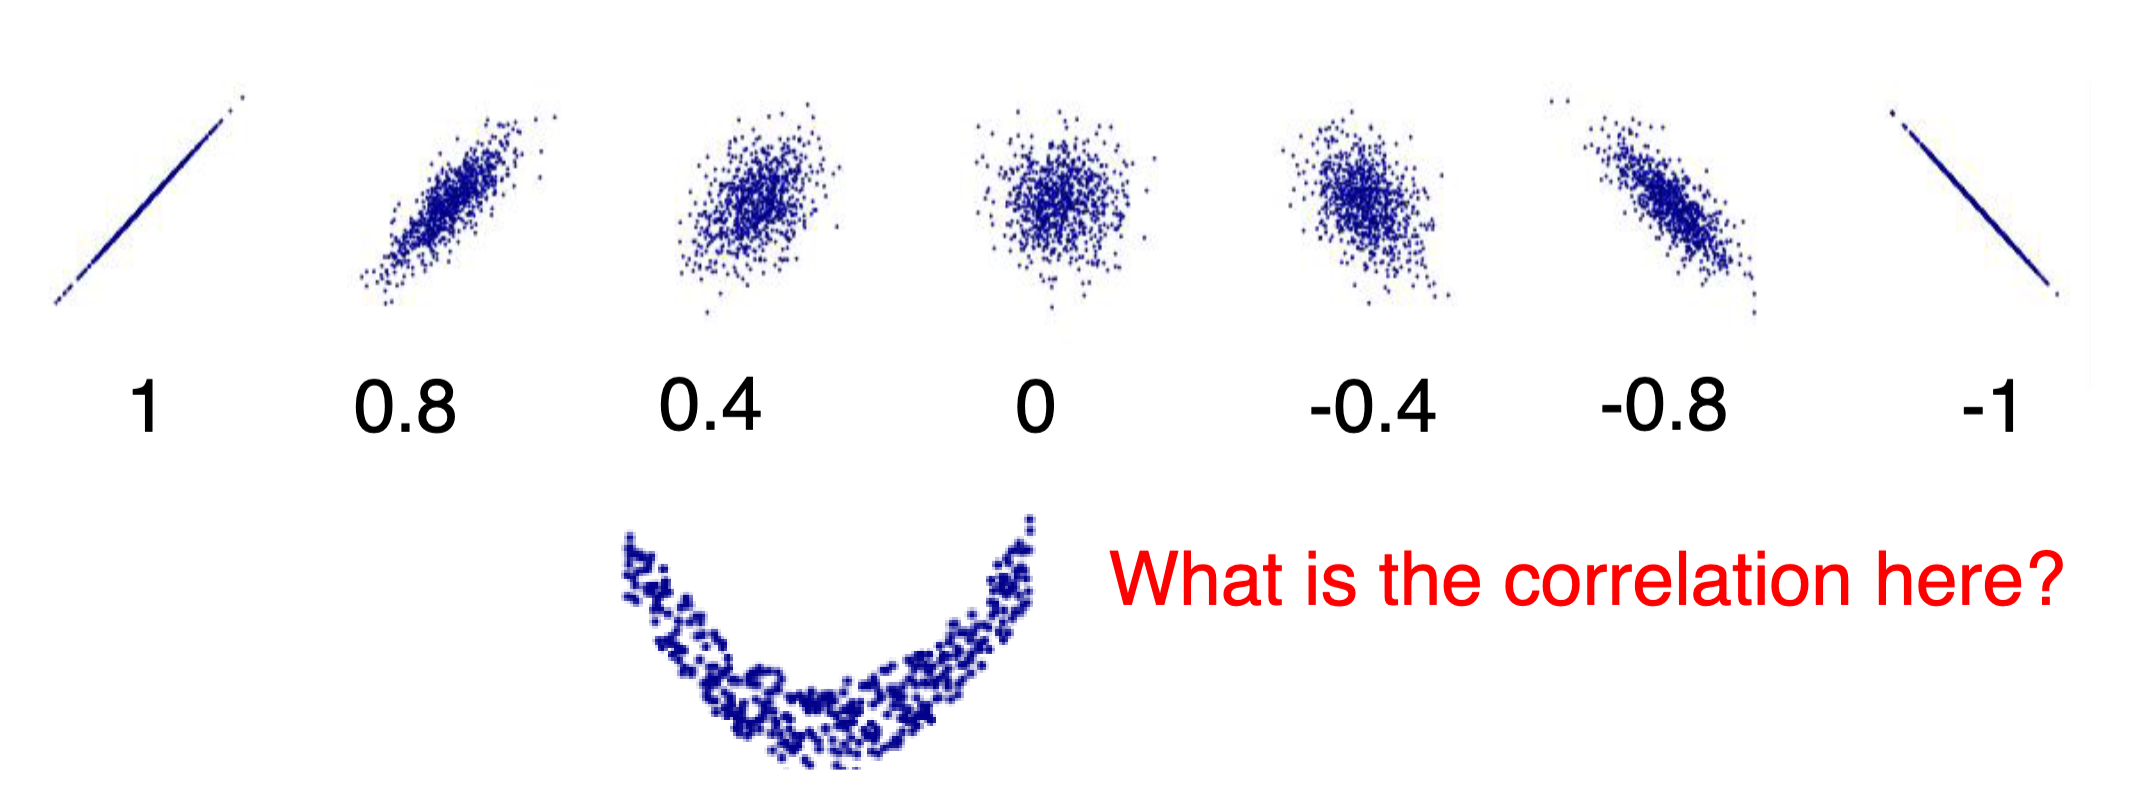
\includegraphics[width=\textwidth/2]{4.png}
\end{itemize}
\begin{note}
  \begin{itemize}
    \item Pearson correlation coefficient is sensitive to
    outliers
    \item It is not robust to outliers
    \item It is not a good measure of correlation for
    non-linear relationships
  \end{itemize}
\end{note}
\section{Feature Analysis: Probability Recap}
This is mathematical so we first
we need to make sure everyone
has the same understanding and
intuition for notation
\subsection{Random Variables}
\begin{itemize}
  \item Random variable (RV) denoted by uppercase letter (e.g. X)
  \item RVs take value assignments X = x where X is a
  \begin{itemize}
    \item Discrete RV if x is in a countable set (binary: x $\in$ {0,1}; or dice)
    \item Continuous RV if x is in an uncountable set (real: x $\in$ Reals)
  \end{itemize}
  \item Write x $\in$ X for possible value assignments of X
  \item For all x, P(X = x) $\in$ [0,1]
  \item P(X = x) is a proper distribution
  \begin{itemize}
    \item Discrete RV: 
    \item 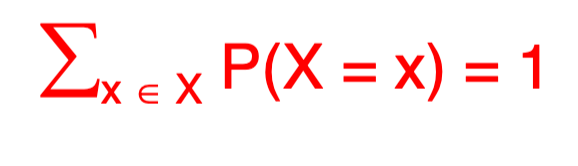
\includegraphics[width=\textwidth/4]{7.png}
    \item Continuous RV:
    \item 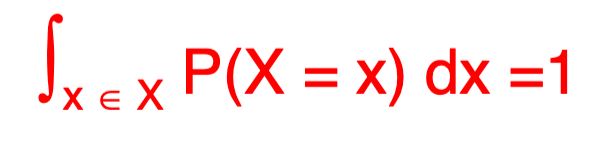
\includegraphics[width=\textwidth/4]{8.png}
  \end{itemize}
  \item Write P(x) for P(X=x), write P(X) for full distribution
  \item Representing probability distributions
  \begin{itemize}
    \item Discrete (finite) RV: tabular
    \item Continuous (infinite) RV: function
  \end{itemize}
\end{itemize}
\subsection{Joint Distributions on RVs}
Aliens in your backyard

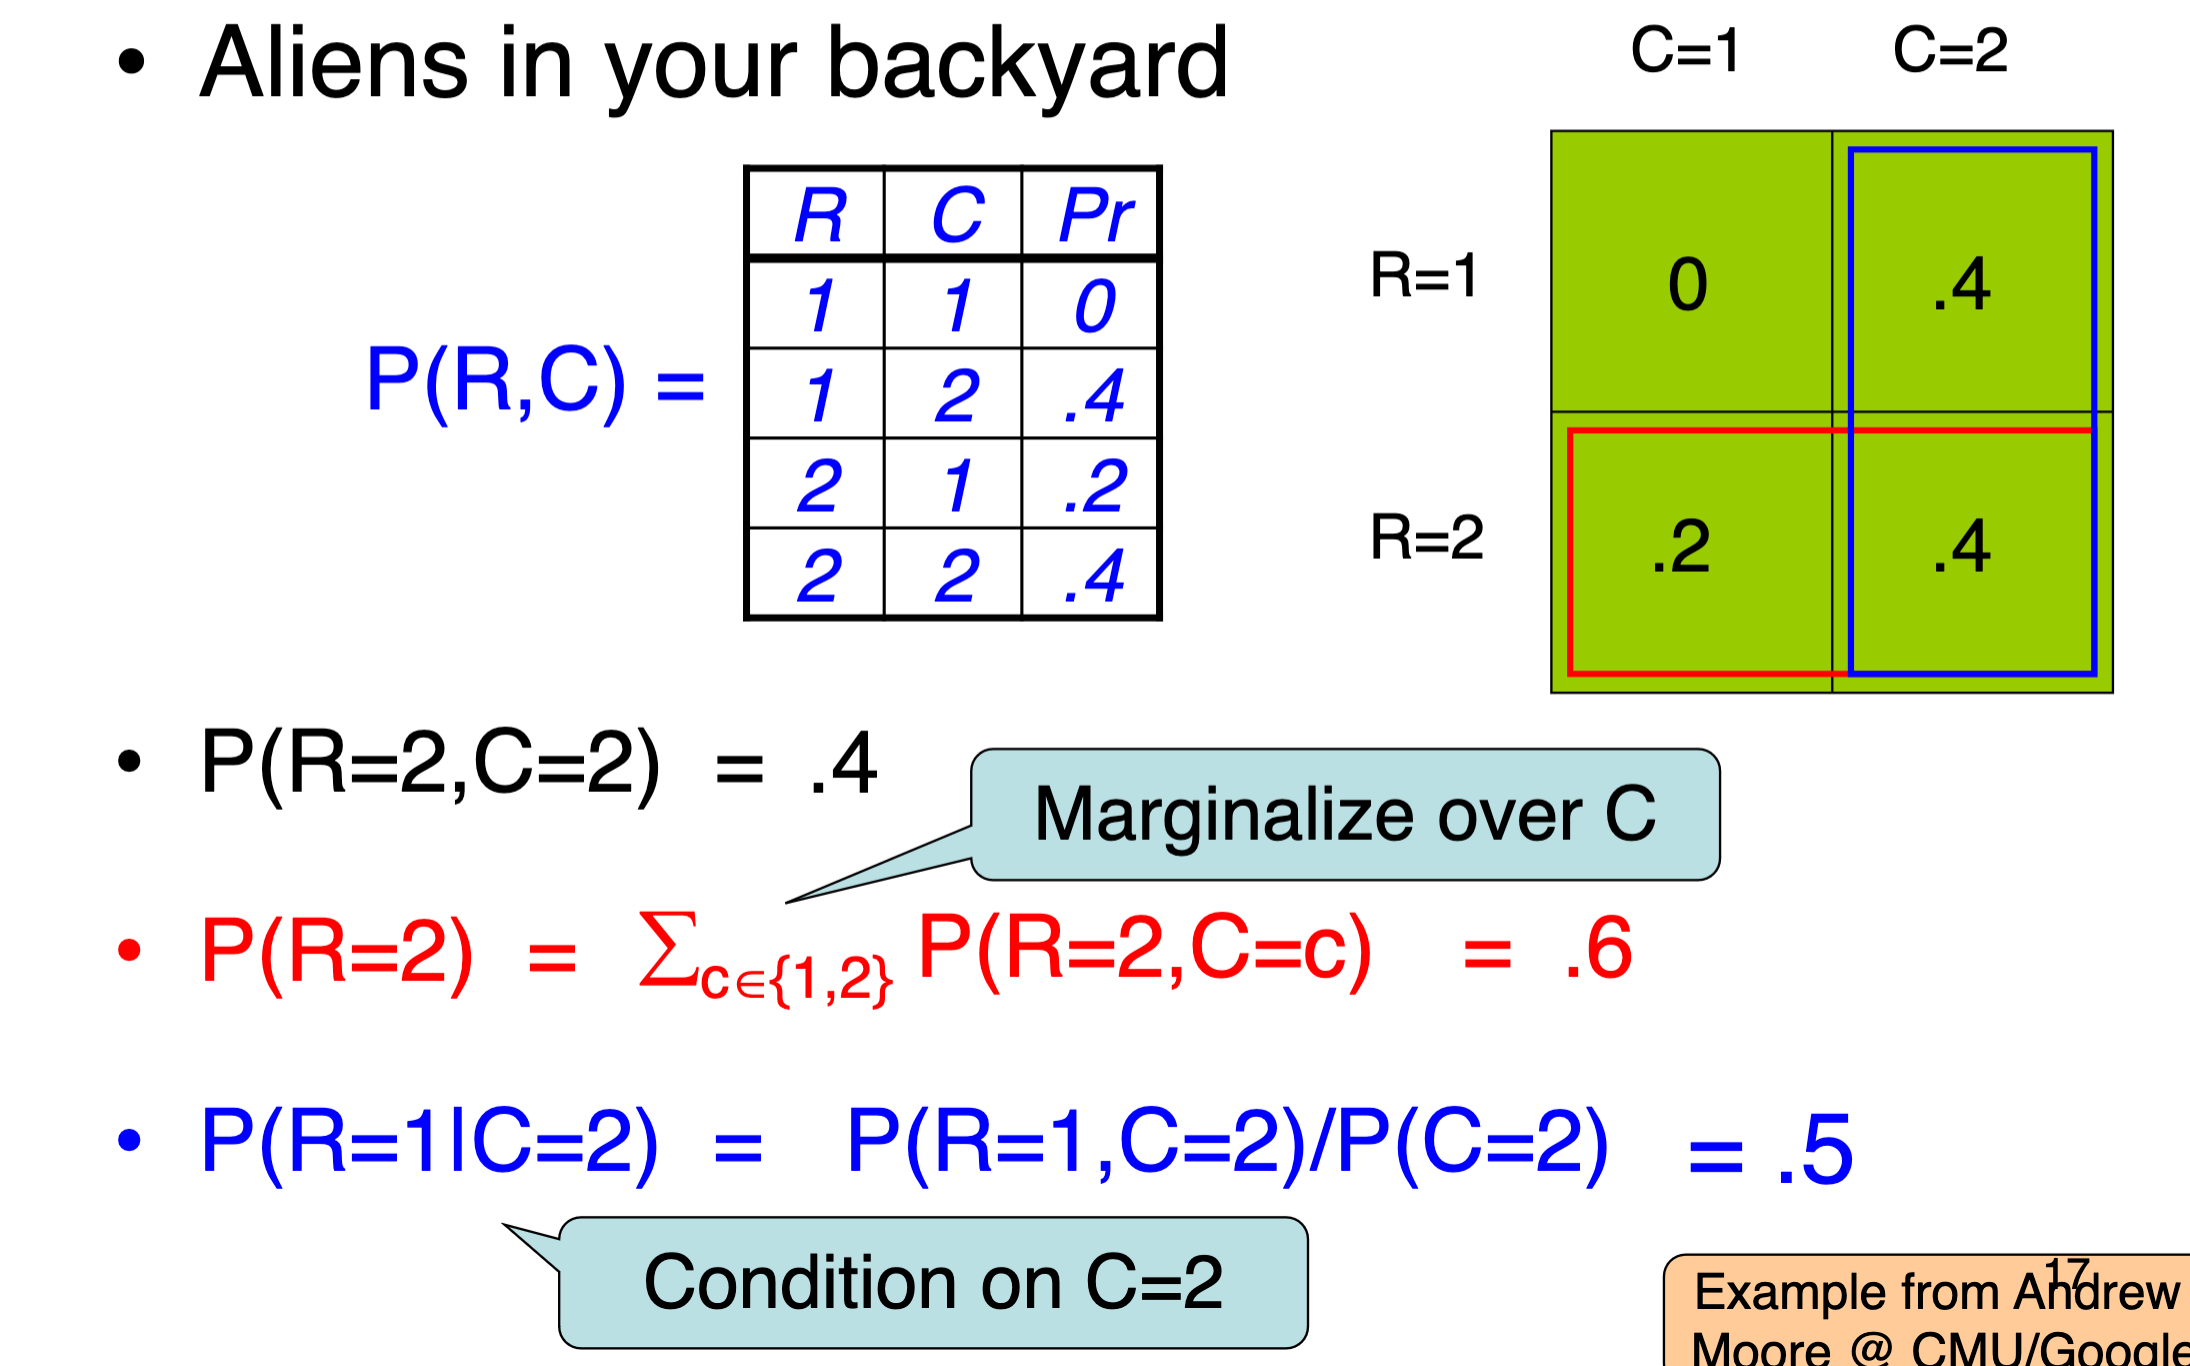
\includegraphics[width=\textwidth]{6.png}
\subsection{Rules of Probability}
\begin{itemize}
  \item Joint and conditional distributions:
  \begin{equation}
    P(X,Y) = P(X|Y)P(Y) = P(Y|X)P(X)
  \end{equation}
  \item Marginalization:
  \begin{equation}
    P(X) = \sum_{y} P(X,Y)
  \end{equation}
  \item Conditional probability \& Bayes rule:
  \begin{equation}
    P(X|Y) = \frac{P(Y|X)P(X)}{P(Y)}
  \end{equation}
\end{itemize}
\subsection{Manipulating Distributions}
\begin{itemize}
  \item Sometimes we don’t just want P(R=1,C=2) = .4
  \item We want to work with full distributions P(R,C)
  \item How to apply previous rules to full distributions?
  \item easy, just do once for each case and store in table
  \item Marginalization:
  \item 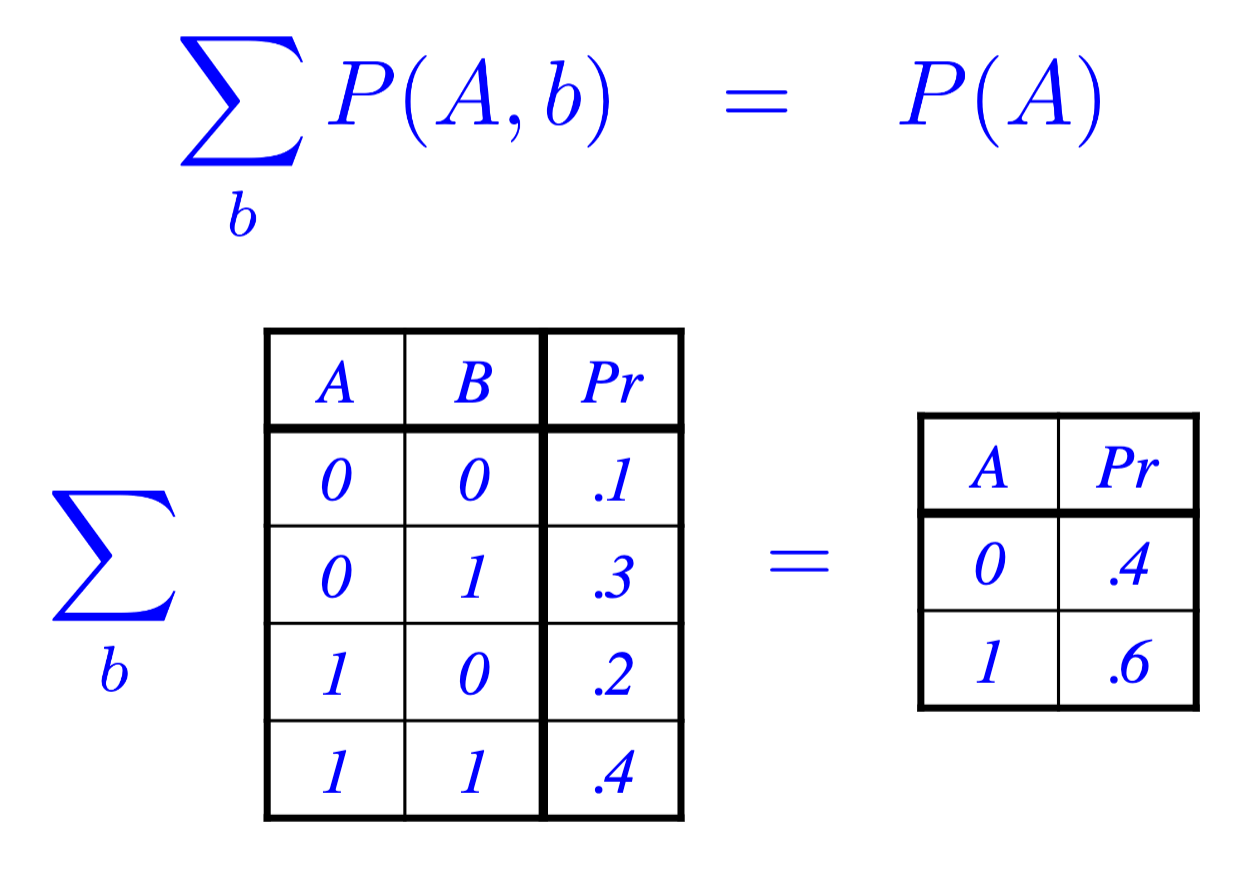
\includegraphics[width=\textwidth/2]{9.png}
  \item Binary Multiplication
  \item 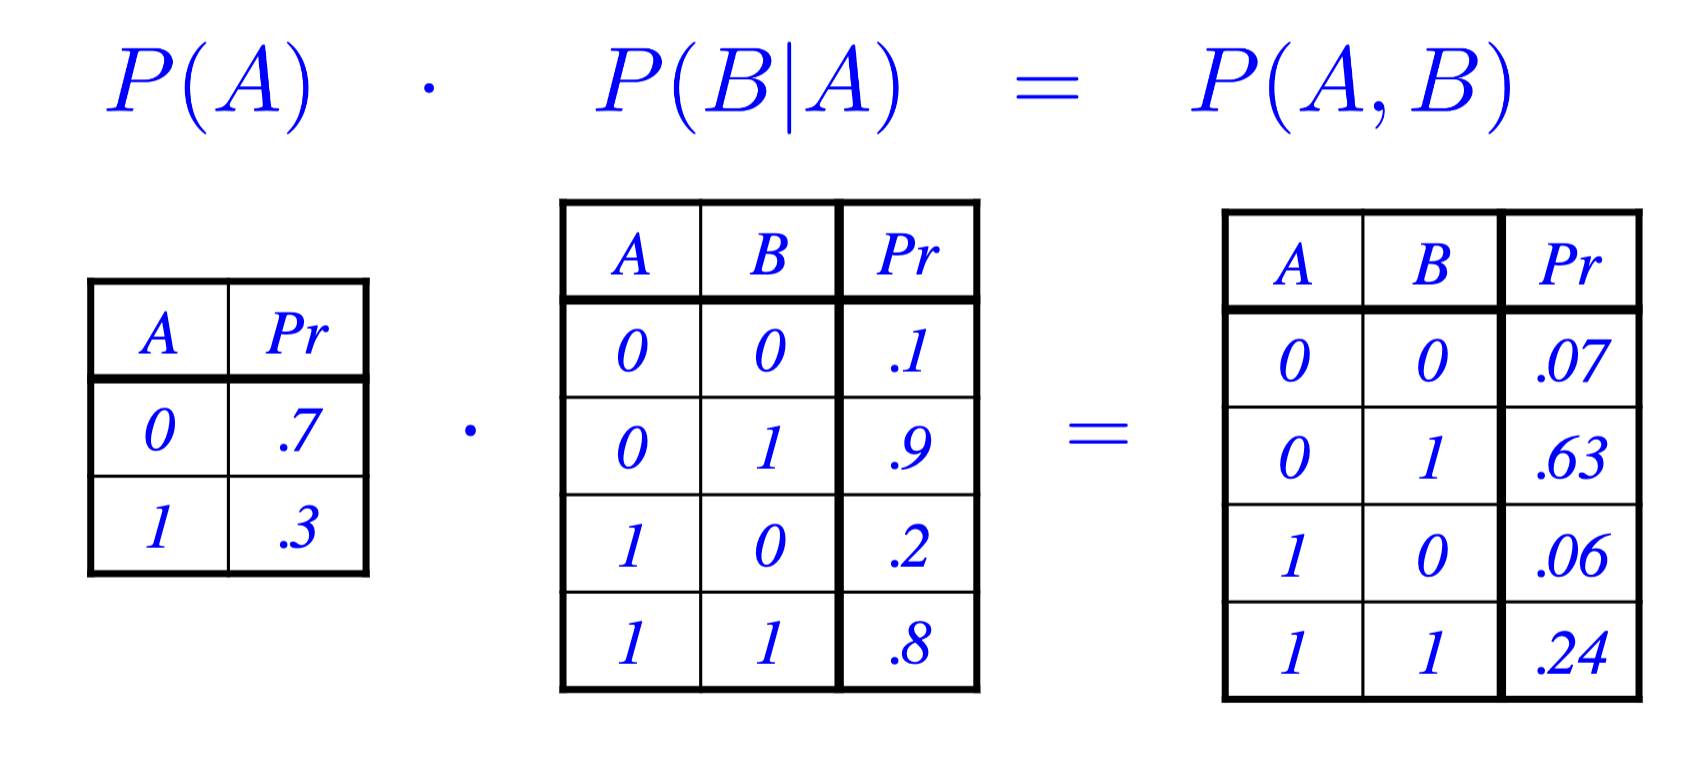
\includegraphics[width=\textwidth/2]{10.png}
\end{itemize}
\section{Feature Analysis}
Frequency, Correlation,
(Pointwise) Mutual Information,
Conditional Entropy
\subsection{Feature Analysis: Frequency}
\begin{itemize}
  \item Always produce summary frequency statistics
  \item Always look at samples of data
  \item 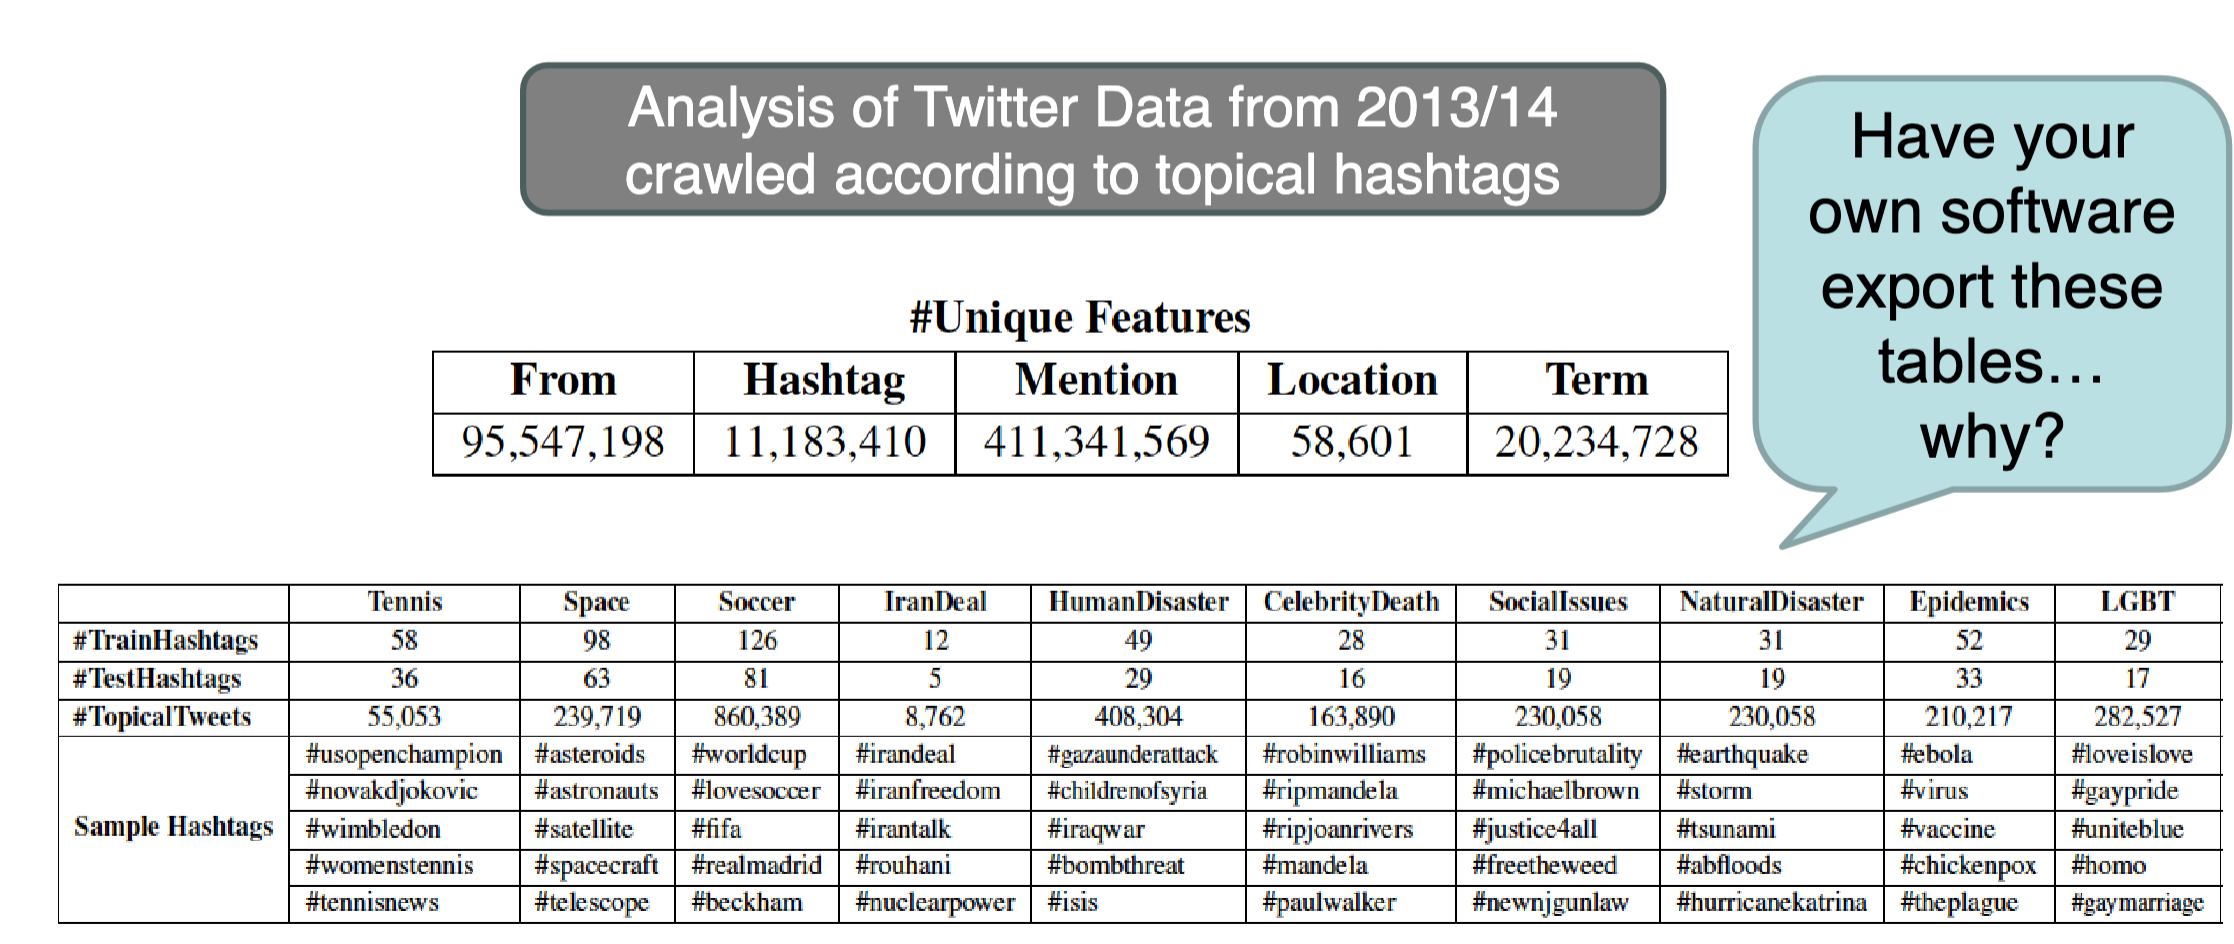
\includegraphics[width=\textwidth/2]{11.png}
\end{itemize}
\subsection{Feature (In)dependence}
Often we want to know whether one feature column
predicts another (bivariate feature analysis)
\begin{itemize}
  \item What do you see here?
  \item How would quantify / visualize / automatically detect this?
  \item 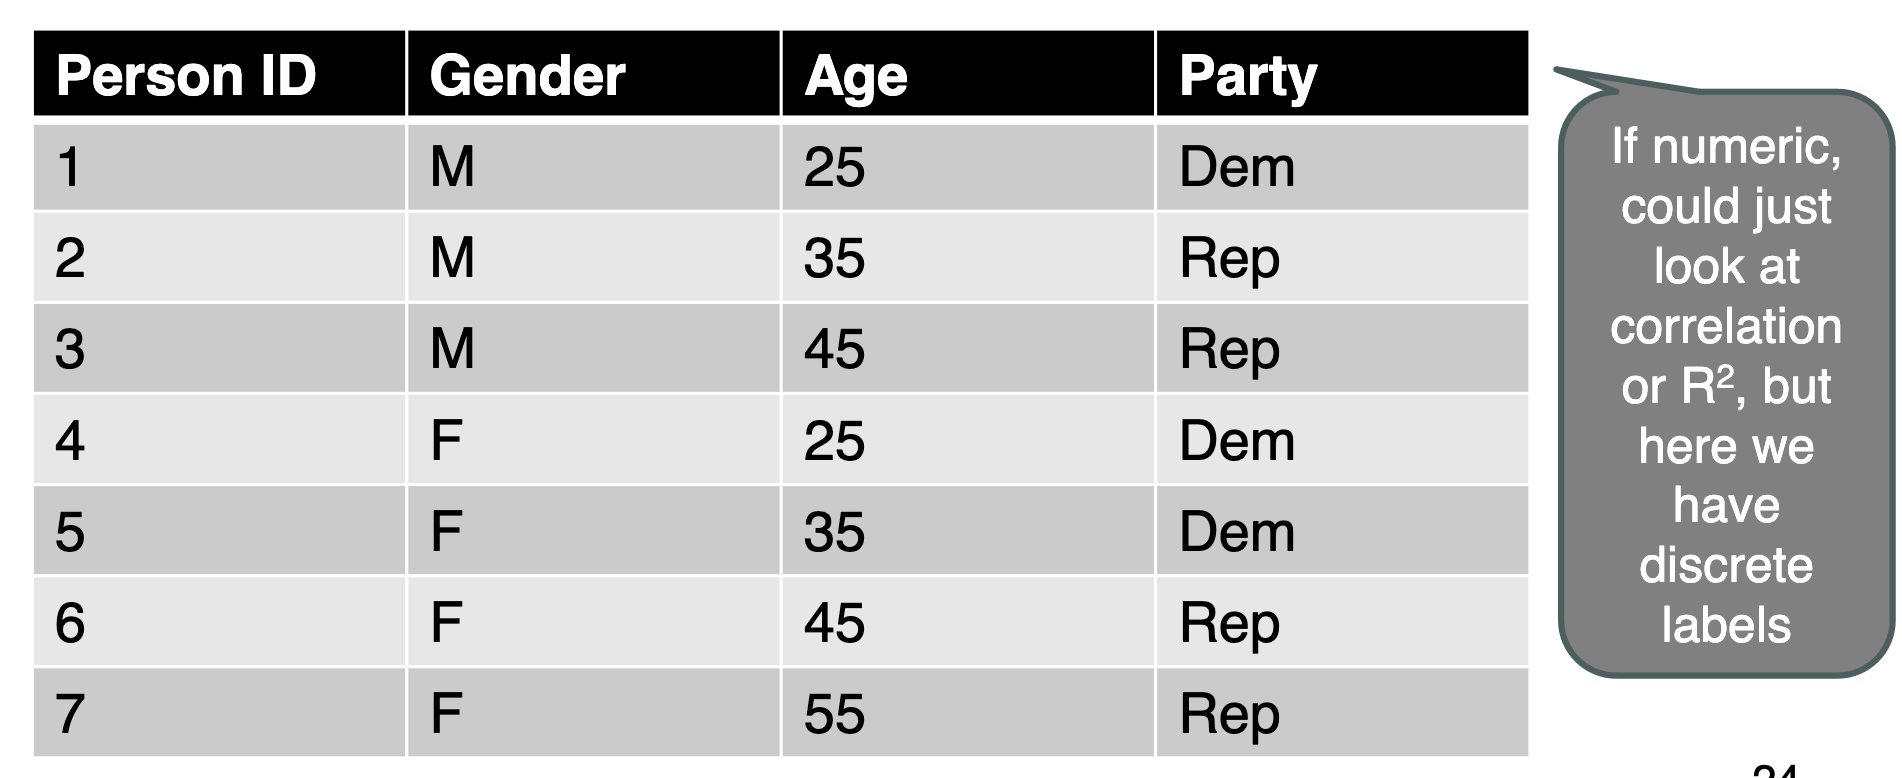
\includegraphics[width=\textwidth/2]{12.png}
\end{itemize}
\subsection{Feature Independence}
\begin{itemize}
  \item X is independent of Y means that knowing Y
  does not change our belief about X
  \item p(X|Y=y) = p(X)
  \item In words: knowing Y=y has no impact on
  our belief in the distribution of X
  \item Occurs if: p(X=x, Y=y) = p(X=x)*p(Y=y)
\end{itemize}
\subsection{Information Theory}
\begin{itemize}
  \item P(X) encodes our uncertainty about X
  \item Some variables are more uncertain that others
  \item 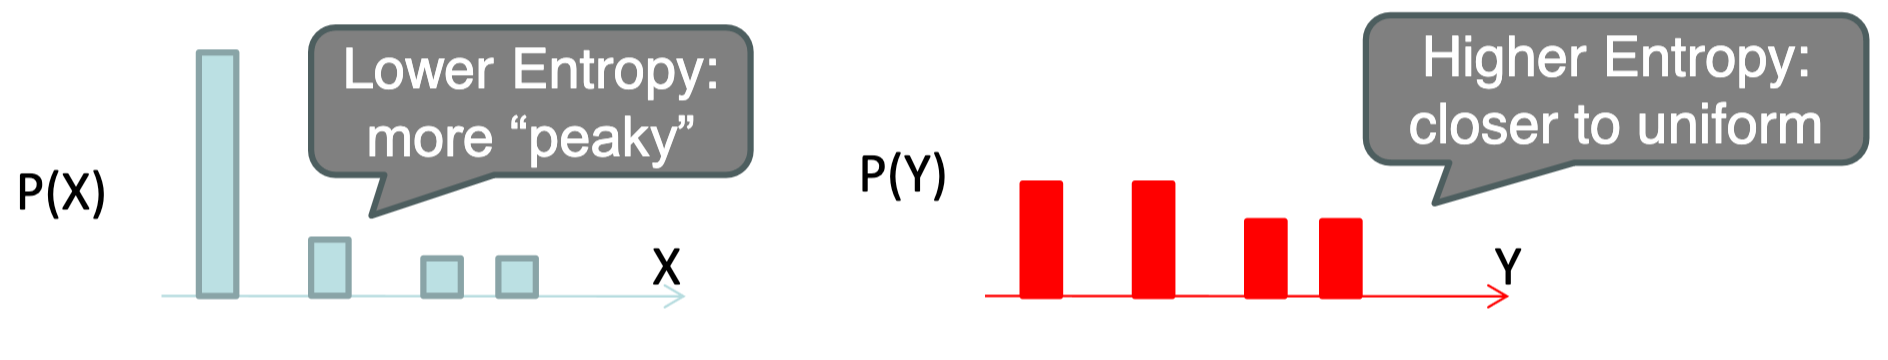
\includegraphics[width=\textwidth/2]{13.png}
  \item How can we quantify this intuition?
  \item Entropy: average number of bits required to encode X
  \item 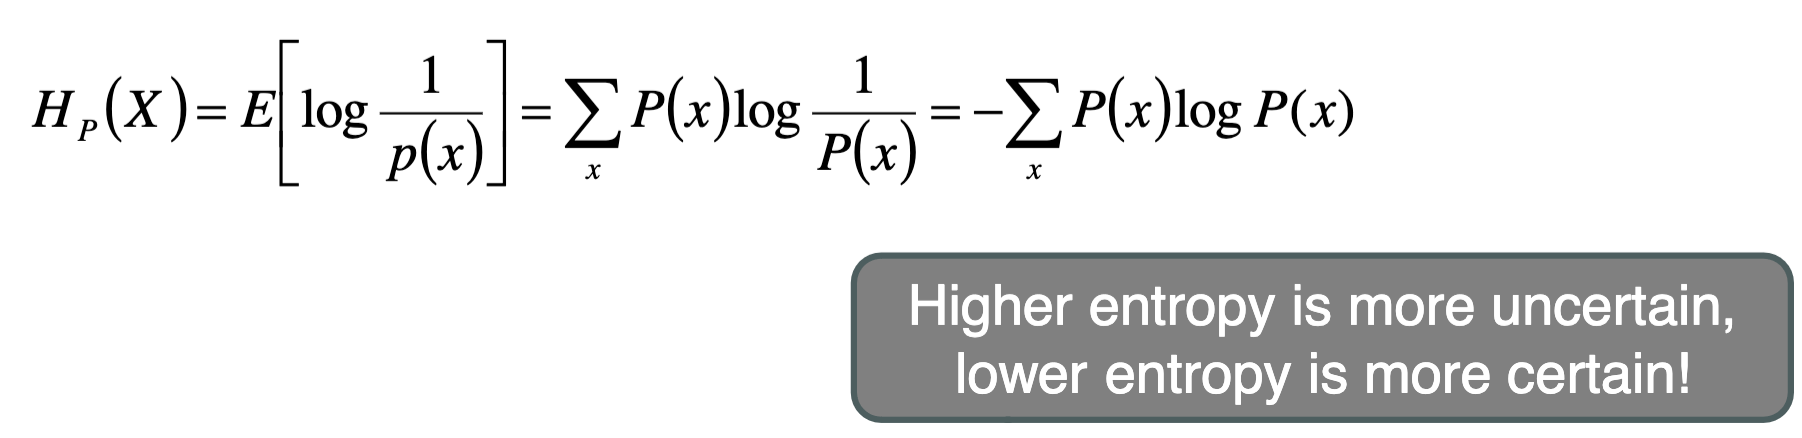
\includegraphics[width=\textwidth/2]{14.png}
  \item In short: low bits, low entropy → low uncertainty
  \item We can define conditional entropy (CE) similarly
  \item 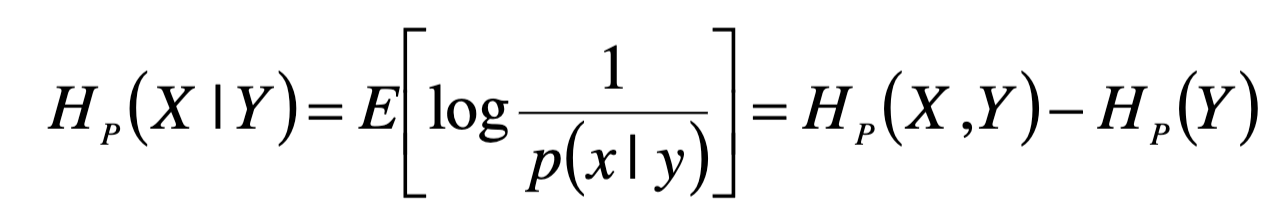
\includegraphics[width=\textwidth/2]{15.png}
  \item i.e. once Y is known, we only need H(X,Y) – H(Y) bits
  \item Higher CE is more uncertain (y is less predictive),
  lower CE is more certain (y is more predictive)
\end{itemize}
\subsection{(Pointwise) Mutual Information}
\begin{note}
  Mutual information is just a test of independence. It only applies to discrete variables. Correlation does not apply to binary variables. If X and Y are non-linear, MI will capture that unlike correlation coefficient.
\end{note}
\begin{itemize}
  \item Mutual Information
  \item 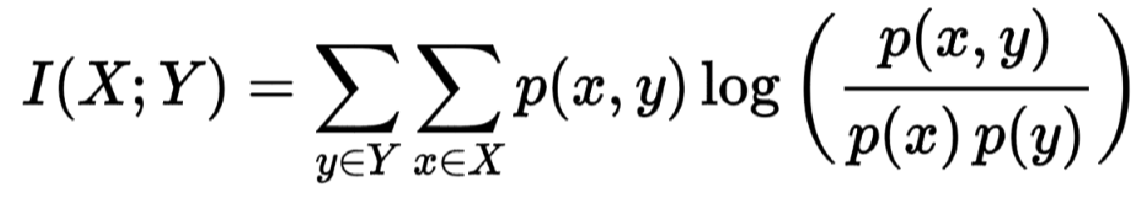
\includegraphics[width=\textwidth/2]{16.png}
  \item For discrete random
  variables: can also
  be generalized to
  continuous case
  \item PMI: target specific values x and y (pointwise)
  \item 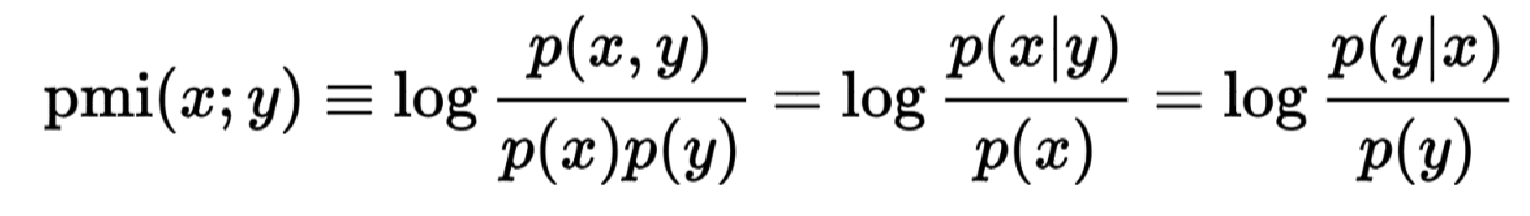
\includegraphics[width=\textwidth/2]{17.png}
  \item Lower MI and PMI → More independent, Higher MI and PMI → More dependent
\end{itemize}
\subsection{Discrete Feature Analysis Summary}
If we look at two feature columns X and Y, can analyze:
\begin{itemize}
  \item MI(X,Y): test independence (fix neither variable)
  \begin{itemize}
    \item MI=0 → independent,
    \item The higher the value, the more dependence
    \item Chi2(X,Y) / Chi-squared(X,Y): independence test similar to MI
  \end{itemize}
  \item CE(X|Y=b): test how well Y=b predicts X (fix Y)
  \begin{itemize}
    \item Low conditional entropy when X is well-predicted, why?
    \item CE=0 → perfect prediction! CE=1 → complete noise!
  \end{itemize}
  \item PMI(X=a,Y=b): test if X=a, Y=b dependent (fix X and Y)
  \begin{itemize}
    \item Hard to interpret absolute numerical meaning (0 is still independent)
    \item Primarily useful when ranking features... why?
  \end{itemize}
\end{itemize}
\subsection{Predictive Feature Analysis:
Mutual Information (MI) or Pointwise MI}
E.g., top 5 term features for Twitter topics
– Use mutual information to know what is
predictive / important
\subsection{Mean, Median, and Power Laws}
\begin{itemize}
  \item A lot of human data is power law (income, \#friends)
  \item Discrete power law (Zipf) for freq f:
  \item 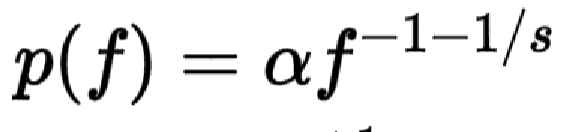
\includegraphics[width=\textwidth/5]{18.png}
  \item Continuous power law:
  \item 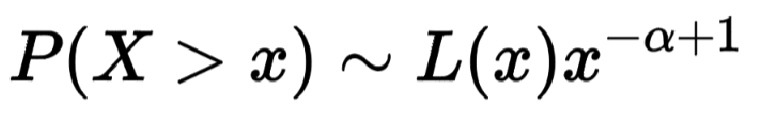
\includegraphics[width=\textwidth/4]{19.png}
  \item E.g., Probability
  mass of
  population with
  different income
  levels, or \#friends
  on Facebook
  \item 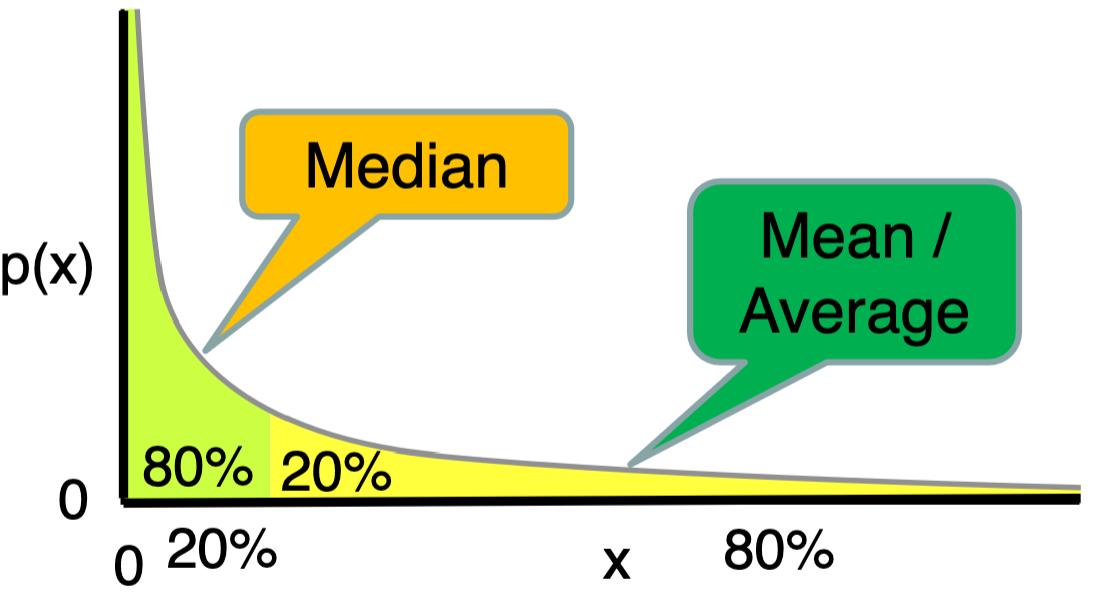
\includegraphics[width=\textwidth/2]{20.png}
  \item Not symmetric like Gaussian, mean $\neq$ median
  \item I.e., the average case is much closer to the max case!
  \item 80/20 rule: top 20\% of values account for 80\% of mass
\end{itemize}
\subsection{Box Plots}
Most data is not Gaussian, often power law or log-Normal

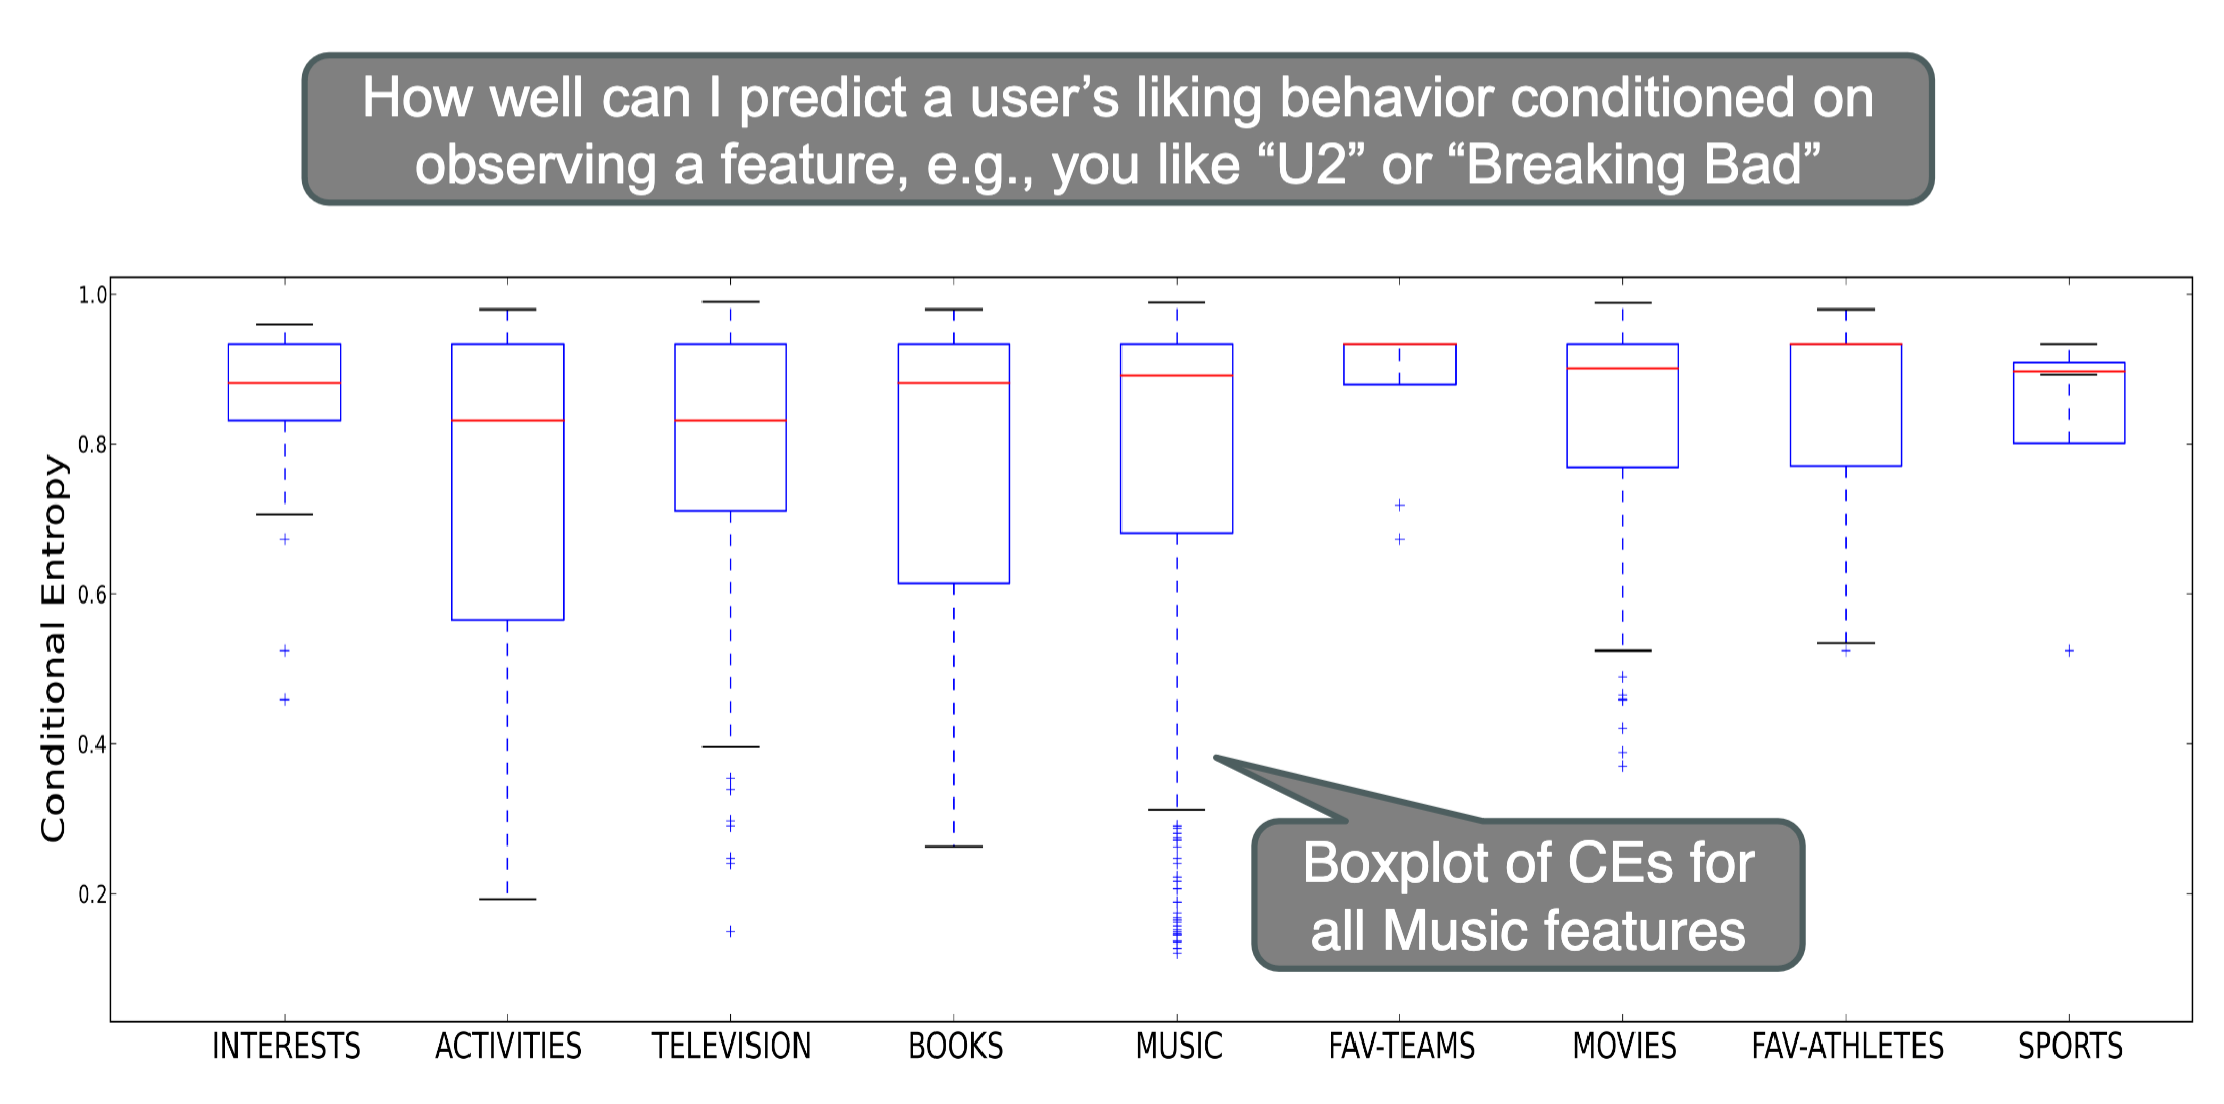
\includegraphics[width=\textwidth]{21.png}

An example where most informative = mean
informative (but not median)... why?

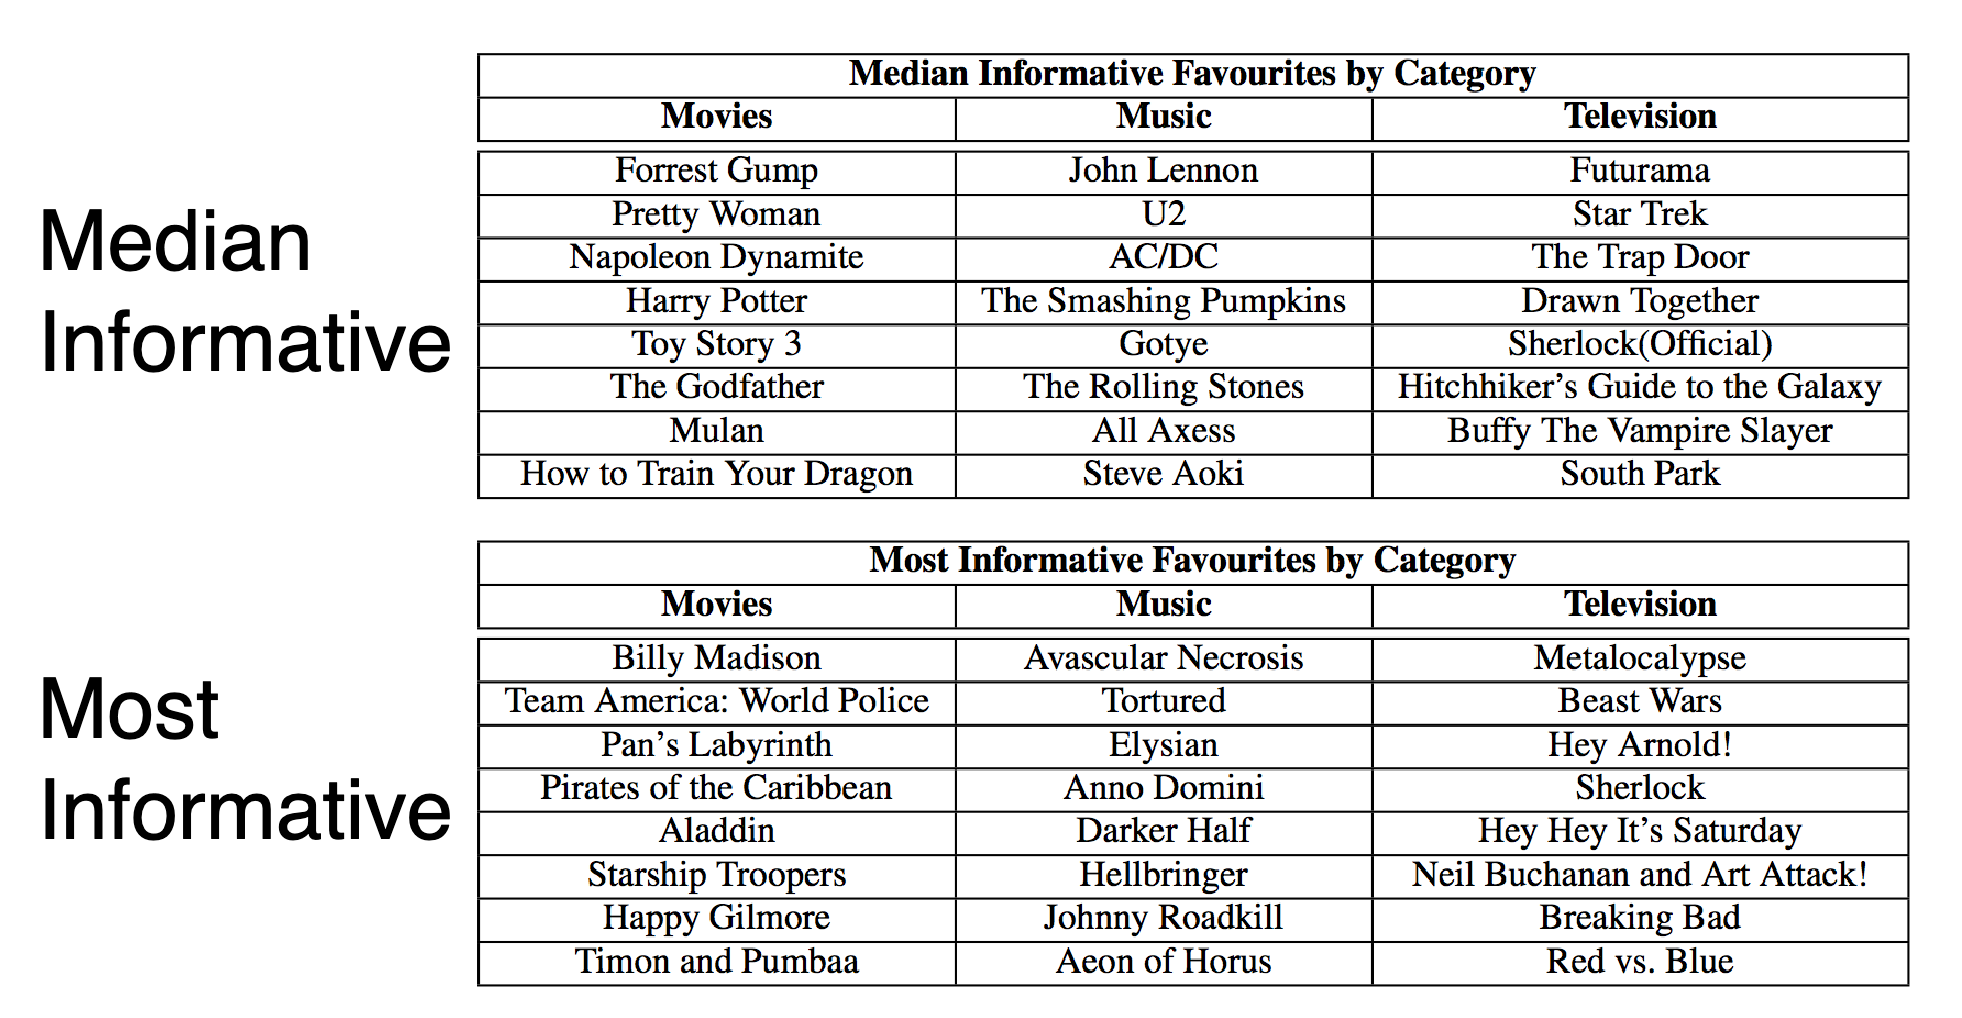
\includegraphics[width=\textwidth]{22.png}
\begin{itemize}
  \item Median favorites were largely generic
  \item Most informative (max $\approx$ avg) were largely specialized
\end{itemize}
\subsection{Violin Plots}
Compactly show full distributions side-by-side. Like compact histogram, can show bimodality unlike Boxplot

Plot of tooth length vs. vitamin C dose

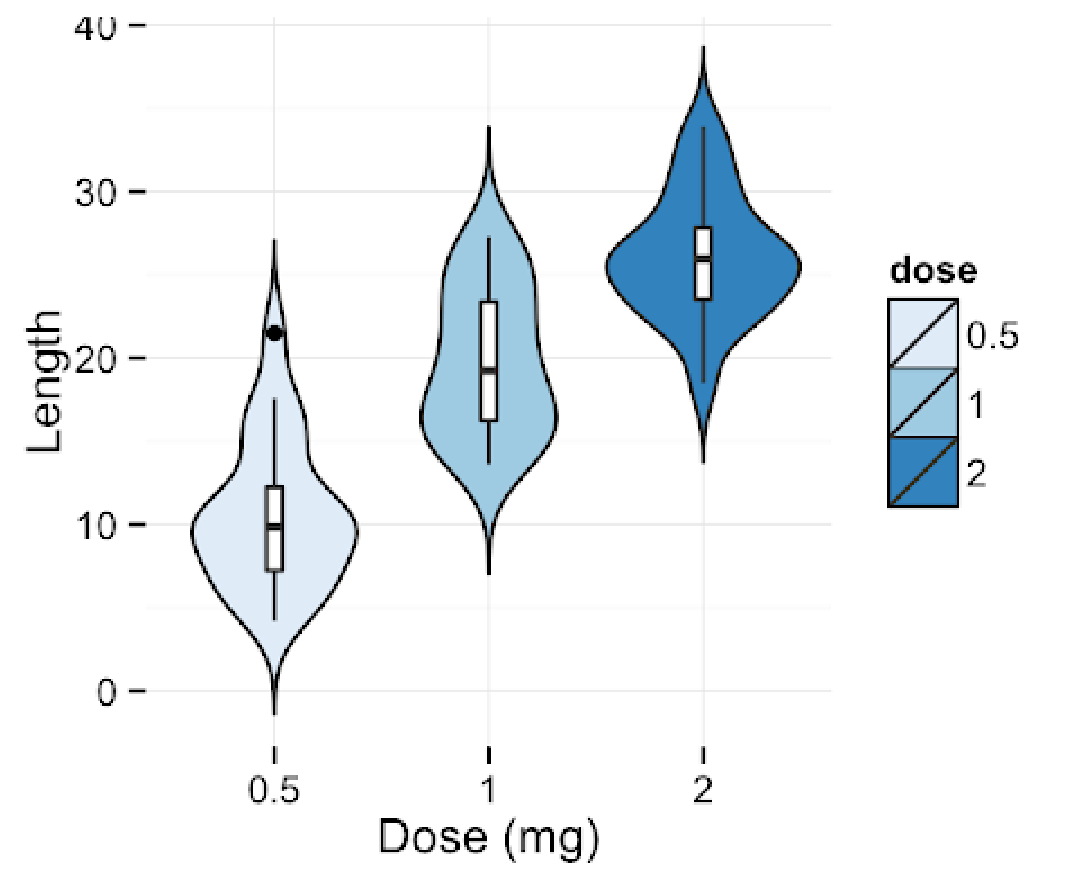
\includegraphics[width=\textwidth/2]{23.png}
\subsection{Discrete Heatmaps}
Better than a table... visualize numbers!

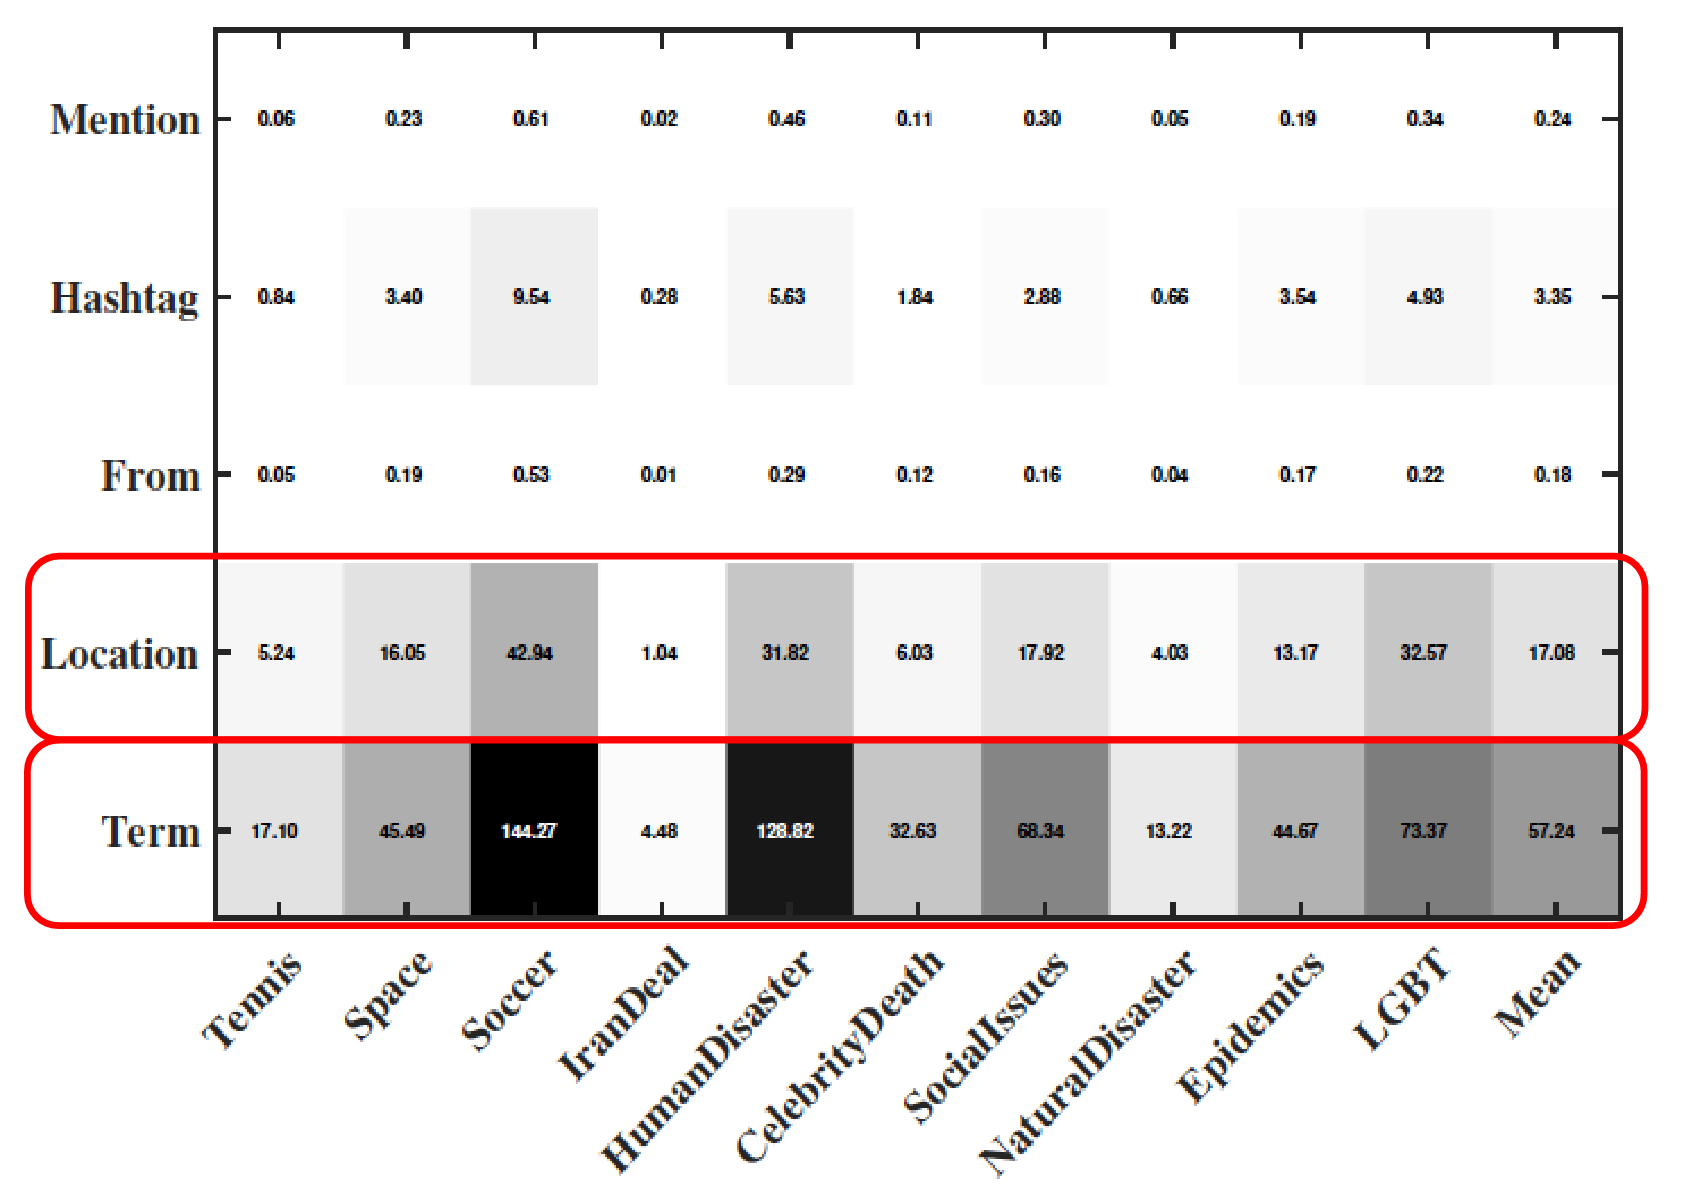
\includegraphics[width=\textwidth]{24.png}
\subsection{Scatterplots: don’t need linear relationship to
be informative!}
\begin{itemize}
  \item Large groups tend not to be predictive
  \item Most informative groups were small
\end{itemize}
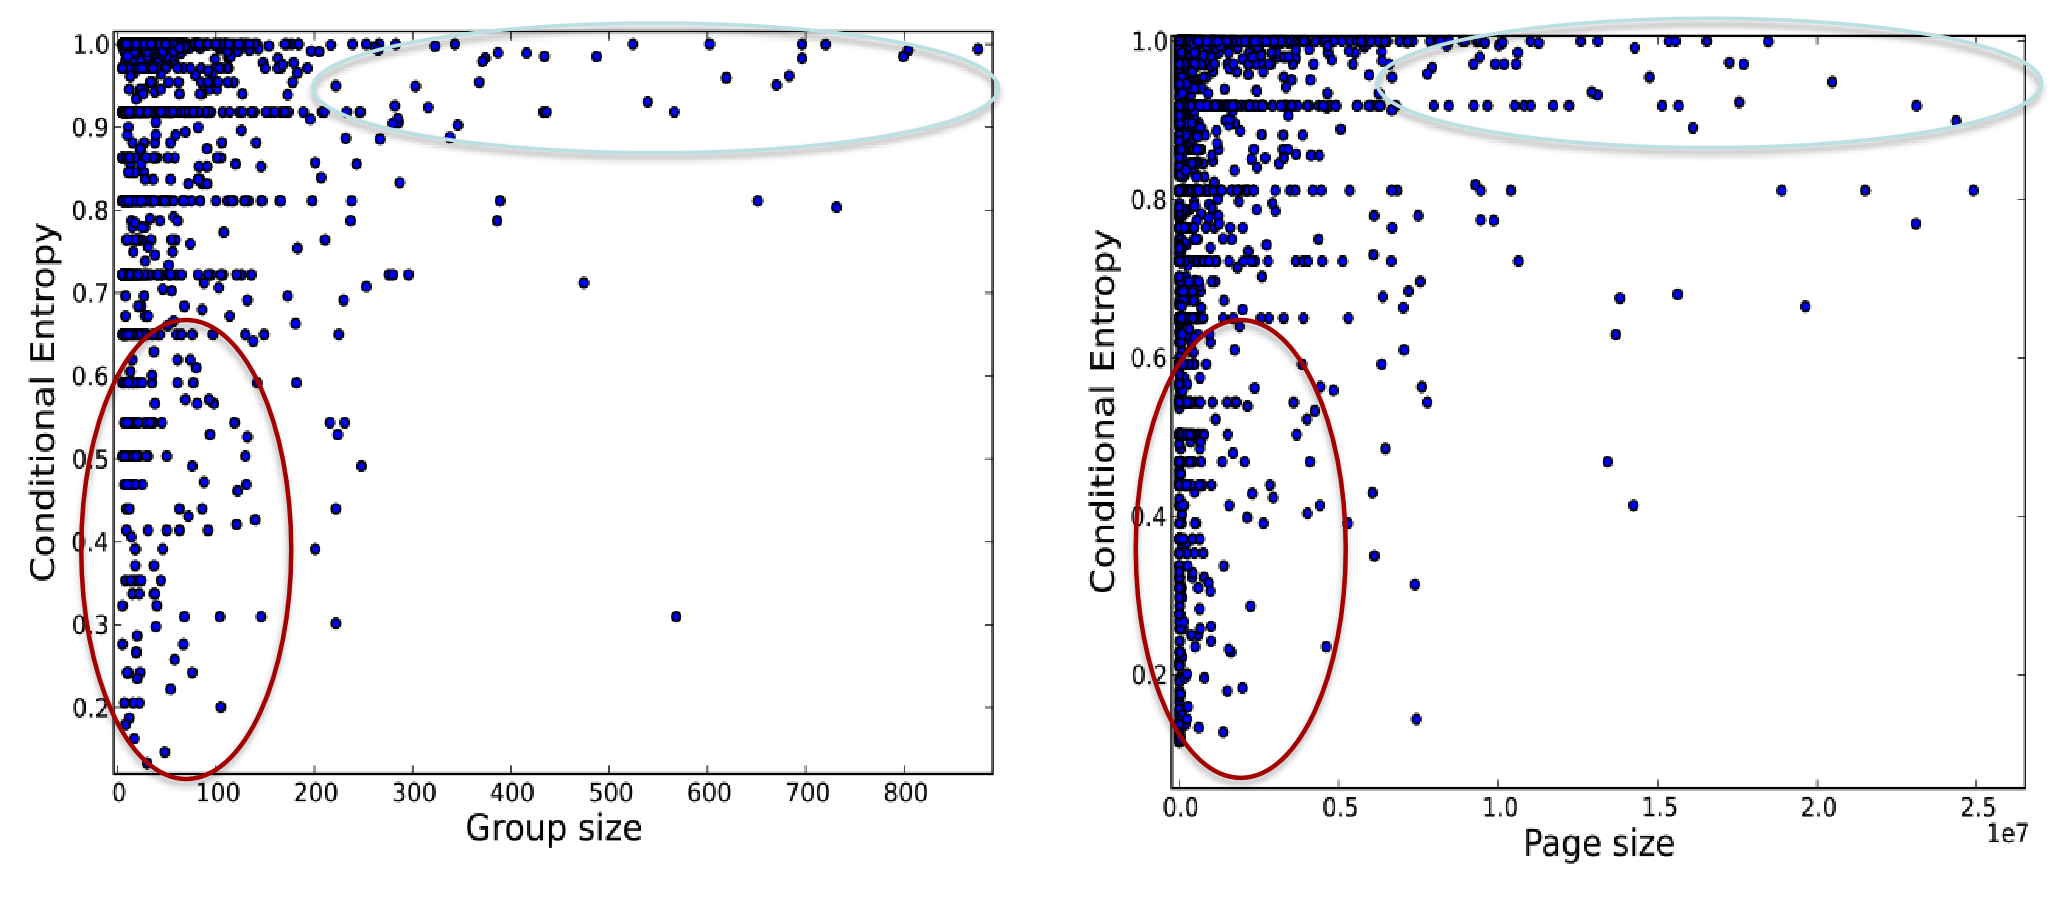
\includegraphics[width=\textwidth]{25.png}

\subsection{Heatmaps / Density Plots}
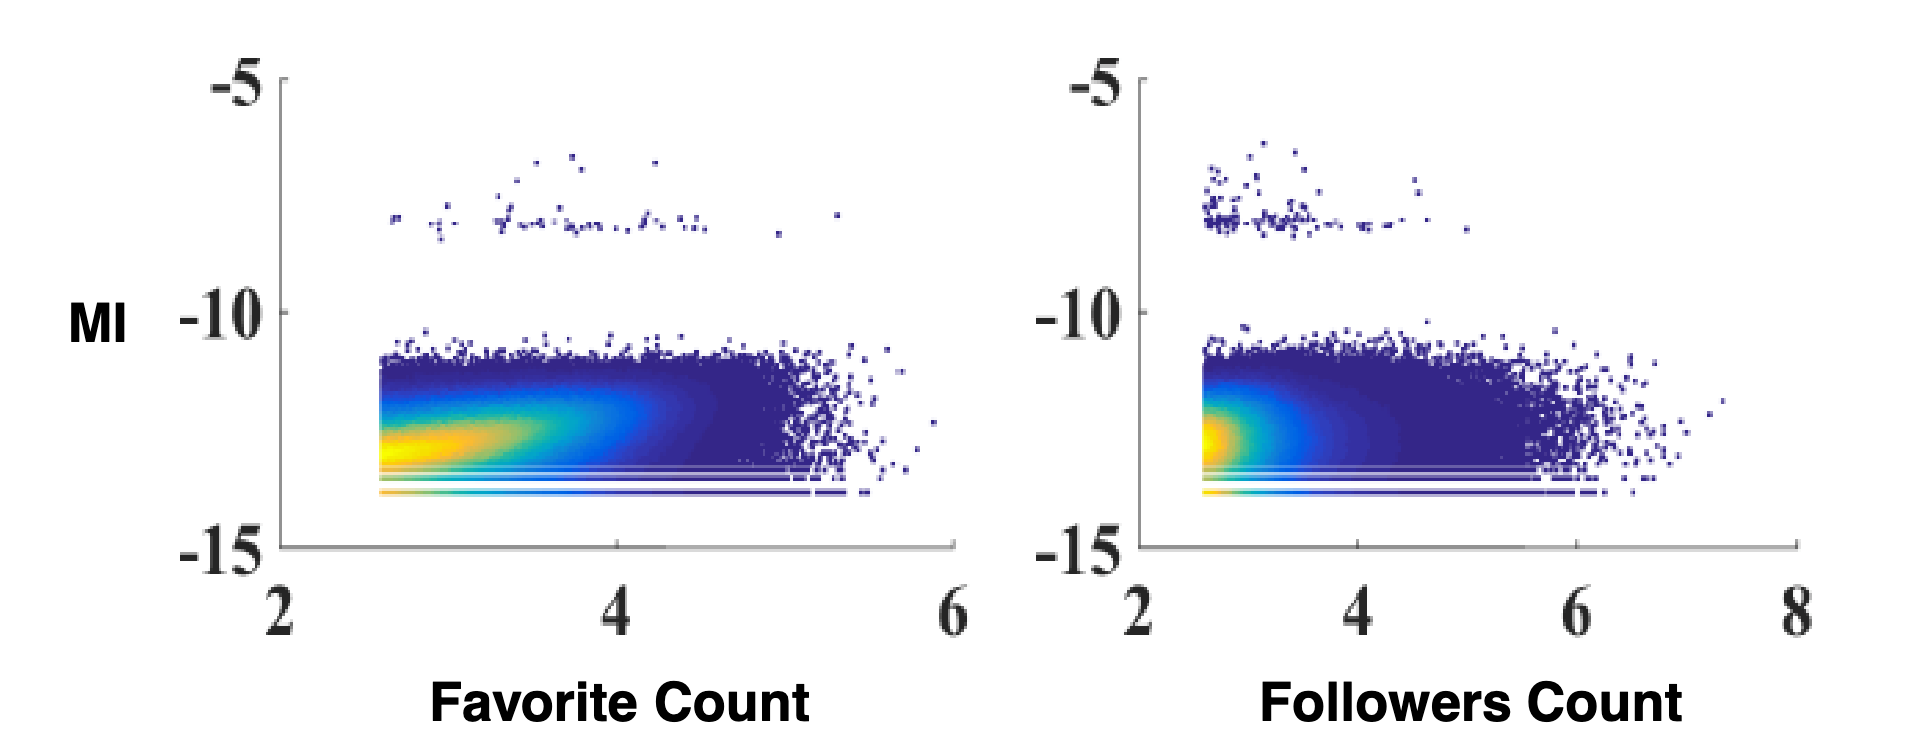
\includegraphics[width=\textwidth]{26.png}

Important to use when points in a scatterplot
are dense and do not reflect density

\subsection{Bubble Plots}
Sometimes scatterplots not
dense enough for a heatmap

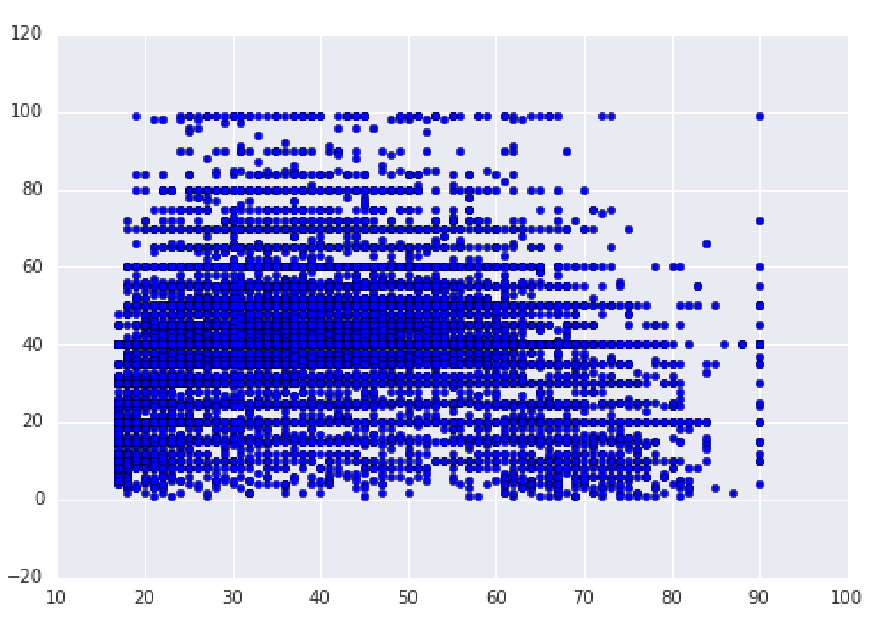
\includegraphics[width=\textwidth/2]{27.png}
\begin{itemize}
  \item And may have a third data
  dimension
  \item So don’t want density=color
\end{itemize}

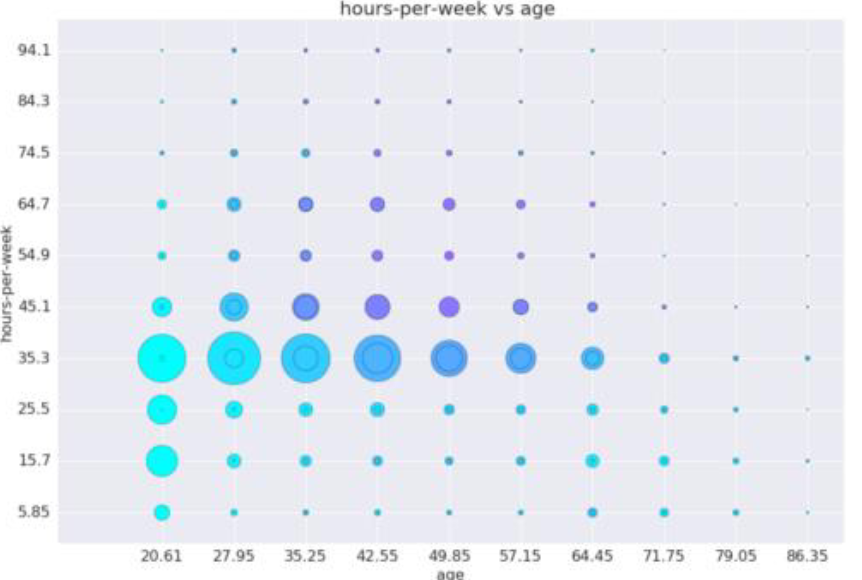
\includegraphics[width=\textwidth/2]{28.png}

Enter the bubble plot
\begin{itemize}
  \item X-axis: age
  \item Y-axis: hours worked per week
  \item Bubble size is relative mass
  (density in a heatmap)
  \item Color is income (purple=higher)
\end{itemize}
\end{document}